Ce chapitre présente la modélisation complète du système PBADS, incluant l'analyse des besoins, la définition des objectifs, la méthodologie adoptée, et la modélisation conceptuelle avec les diagrammes UML.

\section{Modélisation du système}

Cette section présente les diagrammes de modélisation qui illustrent l'architecture et les interactions du système PBADS.

\subsection{Contexte général}

\subsubsection{Situation actuelle et pratique existante}

Avant le développement de PBADS, l'analyse des comportements personnels reposait principalement sur des méthodes manuelles et fragmentées. Les utilisateurs devaient consigner leurs données quotidiennes dans des tableurs Excel ou des applications mobiles isolées, sans capacité d'analyse approfondie ni de détection automatique des anomalies.

\textbf{Lacunes identifiées dans les solutions existantes :}

\begin{itemize}
    \item \textbf{Absence de détection automatique :} Les utilisateurs devaient identifier manuellement les anomalies dans leurs données, ce qui est subjectif et peu fiable.
    \item \textbf{Manque d'analyse prédictive :} Aucun système ne permettait d'anticiper les tendances comportementales ou d'identifier les facteurs contribuant aux anomalies.
    \item \textbf{Recommandations génériques :} Les conseils fournis étaient souvent génériques et non adaptés au profil spécifique de chaque utilisateur.
    \item \textbf{Fragmentation des données :} Les données étaient dispersées dans différents outils sans vue d'ensemble cohérente.
    \item \textbf{Absence de notifications proactives :} Les utilisateurs n'étaient pas alertés en temps réel des anomalies détectées.
    \item \textbf{Manque de visualisation interactive :} Les outils existants offraient peu de capacités de visualisation et de filtrage temporel des données.
\end{itemize}

\textbf{Objectif de la solution}

L'objectif principal est de fournir un système intégré de détection d'anomalies comportementales qui automatise l'analyse des données quotidiennes des utilisateurs et génère des insights actionnables. La solution PBADS doit permettre la saisie structurée des données quotidiennes, la détection automatique des anomalies à l'aide d'algorithmes d'apprentissage automatique non supervisés, la génération d'alertes intelligentes avec identification des facteurs contribuant à l'anomalie, et la production de recommandations personnalisées via l'intégration avec Google Gemini AI.

\subsection{Enjeux et objectifs}

Les enjeux majeurs de PBADS sont : détection automatique des anomalies comportementales, génération de recommandations personnalisées, notifications en temps réel, et visualisation interactive des données. Ces enjeux se traduisent par les objectifs concrets suivants :

\begin{itemize}
    \item \textbf{Gestion des données quotidiennes :} Saisie structurée des habitudes de vie (sommeil, activité physique, alimentation, hydratation, étude, humeur).
    \item \textbf{Détection automatique d'anomalies :} Utilisation d'algorithmes ML (Isolation Forest, One-Class SVM) pour identifier les écarts par rapport aux comportements normaux.
    \item \textbf{Génération d'alertes intelligentes :} Création automatique d'alertes avec niveaux de sévérité (NORMAL, LOW, MEDIUM, HIGH) et facteurs contribuant à l'anomalie.
    \item \textbf{Recommandations personnalisées :} Intégration avec Google Gemini AI pour générer des suggestions adaptées au profil de chaque utilisateur.
    \item \textbf{Visualisation interactive :} Tableau de bord avec graphiques interactifs (Chart.js) et filtres temporels (semaine, mois, année, tout).
    \item \textbf{Notifications en temps réel :} Système de notifications push (toast) pour alerter les utilisateurs immédiatement.
    \item \textbf{Gestion des utilisateurs :} Interface d'administration pour la gestion des comptes avec contrôle d'accès basé sur les rôles (ADMIN, USER).
\end{itemize}

\subsection{Méthodologie adoptée}

Pour ce projet, nous avons opté pour une méthodologie agile, qui favorise un développement itératif et incrémental. Chaque itération permet de livrer des fonctionnalités prêtes à l'usage tout en recueillant régulièrement des retours des utilisateurs.

\textbf{Le cycle de vie du projet}

Le cycle de vie de notre projet comprend les activités suivantes :

\begin{enumerate}
    \item \textbf{Analyse des besoins et faisabilité :} Identification des besoins fonctionnels et non fonctionnels pour la détection d'anomalies comportementales.
    \item \textbf{Planification et priorisation :} Création du backlog produit, définition des priorités et planification des itérations.
    \item \textbf{Conception :} Élaboration des spécifications de l'architecture microservices, des bases de données et des interfaces utilisateur.
    \item \textbf{Développement :} Implémentation progressive des microservices avec des revues de code et une intégration continue.
    \item \textbf{Tests :} Vérification de chaque fonctionnalité par des tests unitaires, fonctionnels et d'intégration.
    \item \textbf{Documentation :} Rédaction des informations nécessaires à l'utilisation, la maintenance et les futures évolutions.
    \item \textbf{Livraison et déploiement :} Livraison progressive des incréments et mise en production du système.
\end{enumerate}

Cette approche agile assure une meilleure collaboration entre les parties prenantes et une flexibilité accrue face aux changements, tout en maintenant un haut niveau de qualité.

\section{Étude Conceptuelle}

Cette section présente l'étude conceptuelle du système avec les diagrammes UML qui modélisent les interactions et la structure de la solution PBADS.

\subsection{Méthodologie}

L'étude conceptuelle suit une approche structurée basée sur l'analyse des besoins utilisateurs et la modélisation des interactions système. Cette méthodologie permet de capturer les exigences fonctionnelles et non-fonctionnelles, d'identifier les acteurs clés, et de concevoir une architecture cohérente et évolutive.

\subsection{Les acteurs principaux}

Le système PBADS implique plusieurs acteurs aux rôles et responsabilités distincts. Le tableau suivant présente l'ensemble des acteurs identifiés avec leurs fonctionnalités principales.

\begin{table}[H]
\centering
\small
\renewcommand{\arraystretch}{1.3}
\begin{tabular}{|p{3cm}|p{4.5cm}|p{6.5cm}|}
\hline
\textbf{Acteur} & \textbf{Rôle} & \textbf{Fonctionnalités principales} \\
\hline
Utilisateur & Utilisateur standard & Connexion, inscription, saisie des données quotidiennes, consultation du tableau de bord, visualisation des alertes, consultation des recommandations, filtrage des graphiques \\
\hline
Administrateur & Gestionnaire système & Hérite de toutes les fonctionnalités utilisateur + gestion des utilisateurs (CRUD), activation/désactivation des comptes, consultation de tous les utilisateurs \\
\hline
Modèle ML & Système autonome & Entraînement du modèle, chargement du modèle, effectuation d'inférence, détection d'anomalies, stockage et versioning du modèle, évaluation du modèle \\
\hline
\end{tabular}
\caption{Acteurs principaux du système PBADS}
\label{tab:acteurs_principaux}
\end{table}

\subsection{Le diagramme de cas d'utilisation}

Le diagramme de cas d'utilisation ci-dessous présente l'ensemble des fonctionnalités du système PBADS, organisées par acteur et illustrant les relations d'héritage entre l'Administrateur et l'Utilisateur.

\begin{figure}[H]
    \centering
    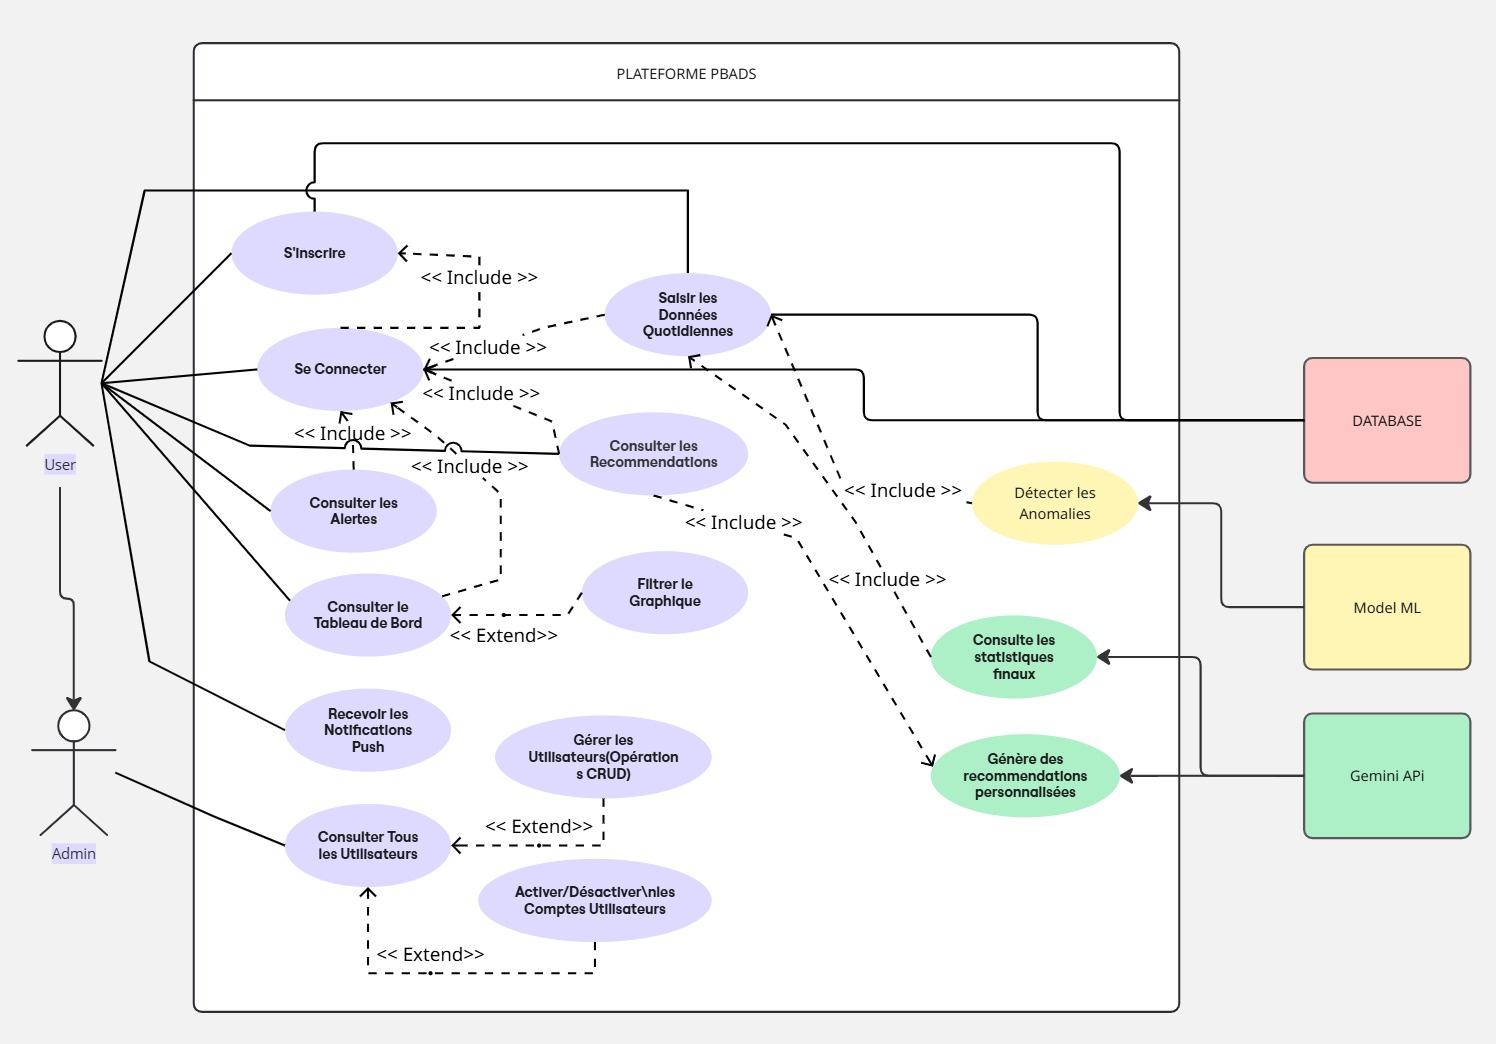
\includegraphics[width=\textwidth]{Figures/pbadsdiags/pbadsusecase.jpg}
    \caption{Diagramme de cas d'utilisation du système PBADS}
    \label{fig:usecase_diagram}
\end{figure}

\textbf{Description du diagramme de cas d'utilisation :}

Le diagramme illustre trois acteurs principaux : \textbf{Utilisateur}, \textbf{Administrateur} (qui hérite de toutes les fonctionnalités utilisateur), et \textbf{Modèle ML}. Les cas d'utilisation sont organisés en trois groupes fonctionnels :

\begin{itemize}
    \item \textbf{Fonctionnalités Utilisateur :} Connexion, inscription, consultation du tableau de bord, saisie des données quotidiennes, consultation des alertes, consultation des recommandations, réception des notifications push, filtrage des graphiques.
    \item \textbf{Fonctionnalités Administrateur :} Gestion des utilisateurs (CRUD), activation/désactivation des comptes, consultation de tous les utilisateurs.
    \item \textbf{Fonctionnalités Modèle ML :} Entraînement, chargement, inférence, détection d'anomalies, stockage, versioning, évaluation.
\end{itemize}

Les relations entre cas d'utilisation incluent des dépendances \texttt{<<include>>} (par exemple, la saisie de données inclut la détection d'anomalies) et des extensions \texttt{<<extend>>} (par exemple, la consultation du tableau de bord peut étendre le filtrage des graphiques).

\subsection{Diagramme de classes}

Le diagramme de classes ci-dessous présente l'architecture complète du système PBADS, illustrant les entités métier principales et leurs relations. Cette modélisation reflète fidèlement l'implémentation technique réalisée avec Spring Boot et JPA.

\begin{figure}[H]
    \centering
    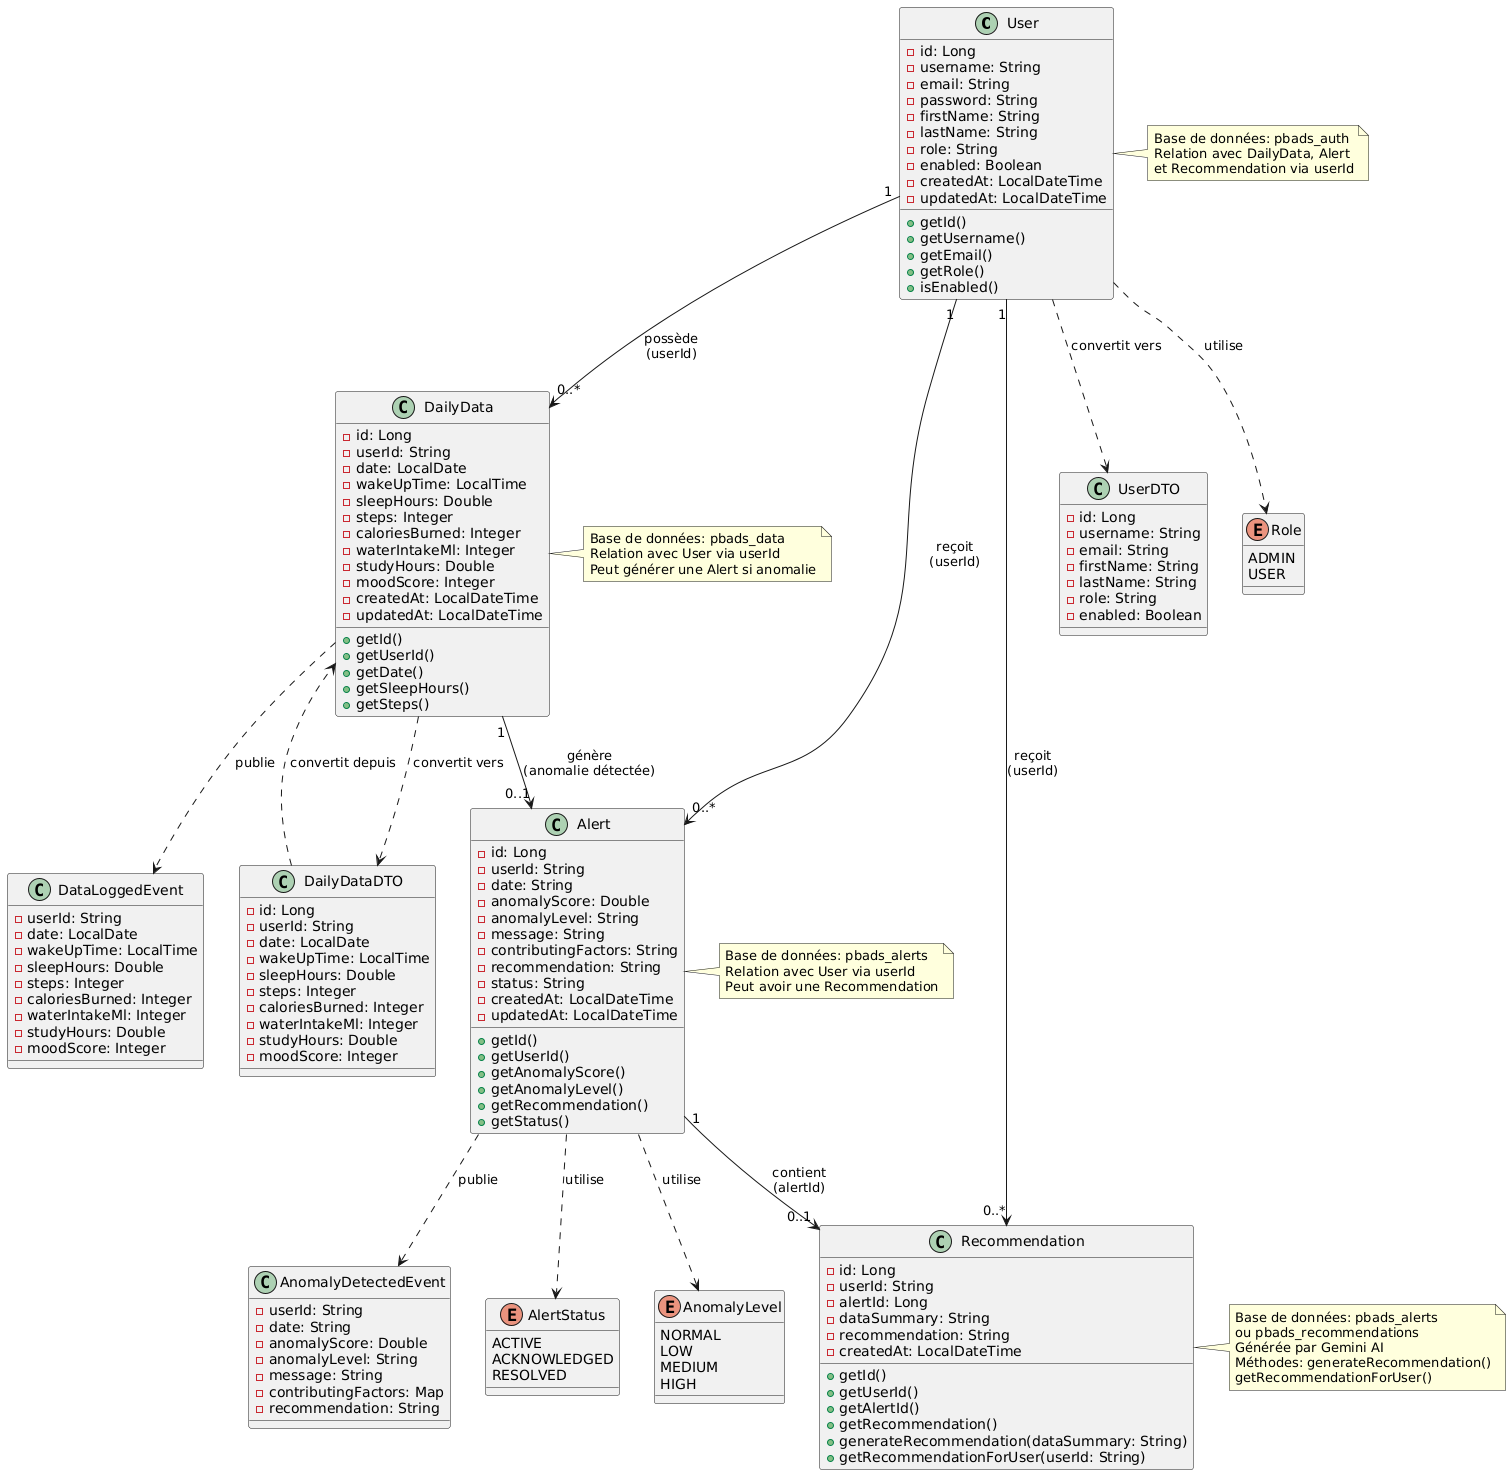
\includegraphics[width=\textwidth]{Figures/pbadsdiags/classdiagram.jpg}
    \caption{Diagramme de classes du système PBADS}
    \label{fig:class_diagram}
\end{figure}

\textbf{Description du diagramme de classes :}

Le modèle de données s'articule autour de trois entités principales : \textbf{User}, \textbf{DailyData}, et \textbf{Alert}. Chaque entité est stockée dans une base de données PostgreSQL distincte selon le principe de l'architecture microservices (une base de données par service).

\textbf{Entités principales :}

\begin{itemize}
    \item \textbf{User :} Gestion des comptes utilisateurs avec authentification JWT, incluant les attributs username, email, password (hashé avec BCrypt), role (ADMIN ou USER), enabled (actif/désactivé), et les timestamps createdAt et updatedAt.
    \item \textbf{DailyData :} Données quotidiennes des utilisateurs avec userId, date, wakeUpTime, sleepHours, steps, caloriesBurned, waterIntakeMl, studyHours, moodScore, et les timestamps createdAt et updatedAt.
    \item \textbf{Alert :} Alertes générées lors de la détection d'anomalies avec userId, date, anomalyScore (0-1), anomalyLevel (NORMAL, LOW, MEDIUM, HIGH), message, contributingFactors (JSON), recommendation (générée par Gemini AI), status (ACTIVE, ACKNOWLEDGED, RESOLVED), et les timestamps createdAt et updatedAt.
    \item \textbf{Recommendation :} Entité représentant les recommandations générées par Google Gemini AI, avec userId, alertId, dataSummary, recommendation, et createdAt. Les méthodes incluent generateRecommendation() et getRecommendationForUser().
\end{itemize}

\textbf{Relations clés :}

Le diagramme illustre les relations cardinales importantes :
\begin{itemize}
    \item Un \textbf{User} (1) peut avoir plusieurs \textbf{DailyData} (0..*) via userId
    \item Un \textbf{User} (1) peut recevoir plusieurs \textbf{Alert} (0..*) via userId
    \item Un \textbf{User} (1) peut recevoir plusieurs \textbf{Recommendation} (0..*) via userId
    \item Une \textbf{DailyData} (1) peut générer une \textbf{Alert} (0..1) si une anomalie est détectée
    \item Une \textbf{Alert} (1) peut avoir une \textbf{Recommendation} (0..1) associée via alertId
\end{itemize}

\textbf{Énumérations :}

Le système utilise plusieurs énumérations pour standardiser les valeurs : \texttt{Role} (ADMIN, USER), \texttt{AlertStatus} (ACTIVE, ACKNOWLEDGED, RESOLVED), et \texttt{AnomalyLevel} (NORMAL, LOW, MEDIUM, HIGH).

Cette architecture garantit l'intégrité des données, la cohérence des relations et la flexibilité nécessaire pour supporter l'évolution future du système.

\subsection{Les diagrammes de séquence}

Cette section présente les flux d'interactions dynamiques entre les différents acteurs du système PBADS. Les diagrammes de séquence suivants décomposent chaque processus en étapes claires, montrant les échanges d'informations entre les acteurs humains et les composants système.

\subsubsection{Scénario : Administrateur interagissant avec la plateforme}

\begin{figure}[H]
    \centering
    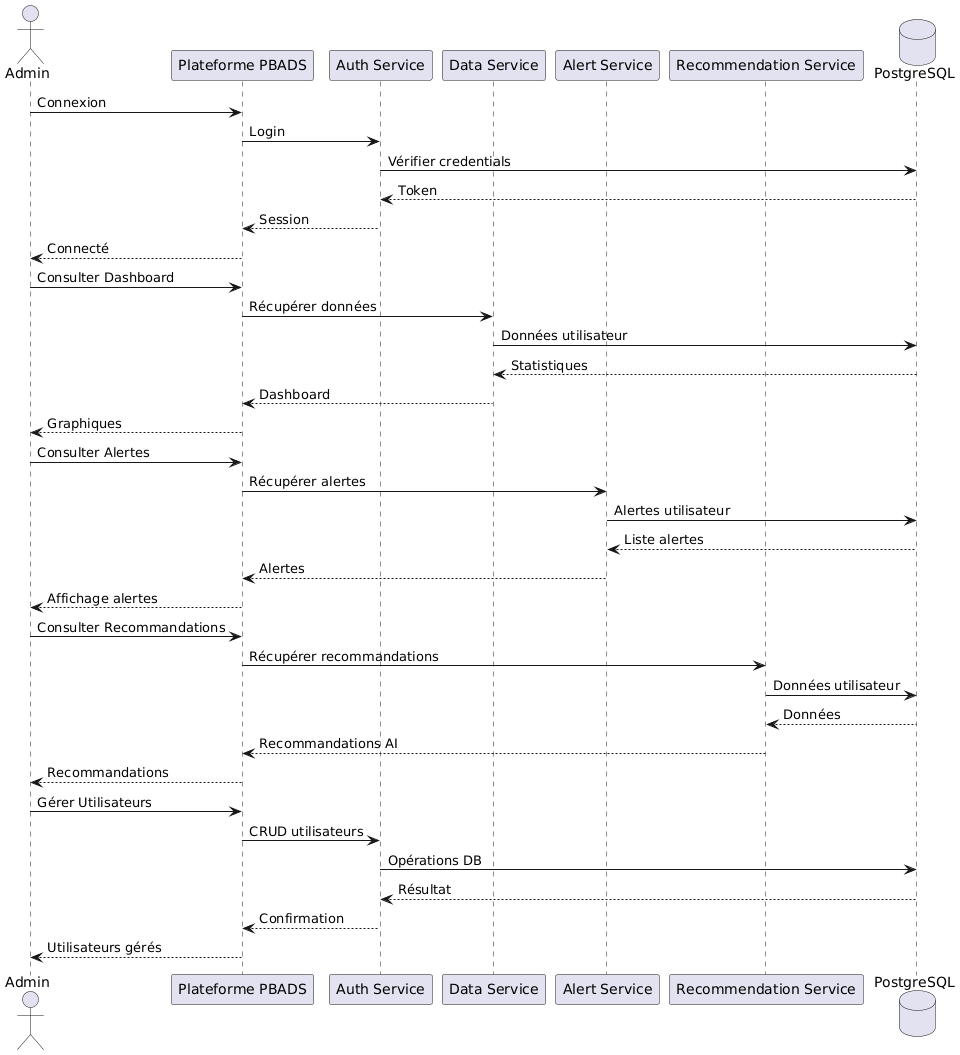
\includegraphics[width=\textwidth]{Figures/pbadsdiags/SequenceAdminPlateform.jpg}
    \caption{Diagramme de séquence - Administrateur interagissant avec la plateforme}
    \label{fig:seq_admin}
\end{figure}

\textbf{Scénario Administrateur (Figure \ref{fig:seq_admin}) :} Ce diagramme illustre les interactions d'un administrateur avec le système PBADS. Le scénario commence par la \textbf{connexion} de l'administrateur via le service d'authentification, qui vérifie les credentials et retourne un token JWT. L'administrateur peut ensuite \textbf{consulter le tableau de bord} en récupérant les données quotidiennes et les recommandations. Il peut également \textbf{consulter les alertes} pour visualiser toutes les alertes générées. Enfin, l'administrateur peut \textbf{gérer les utilisateurs} en effectuant des opérations CRUD (création, lecture, mise à jour, suppression) et activer/désactiver les comptes utilisateurs.

\subsubsection{Scénario : Modèle ML interagissant avec la base de données et la plateforme}

\begin{figure}[H]
    \centering
    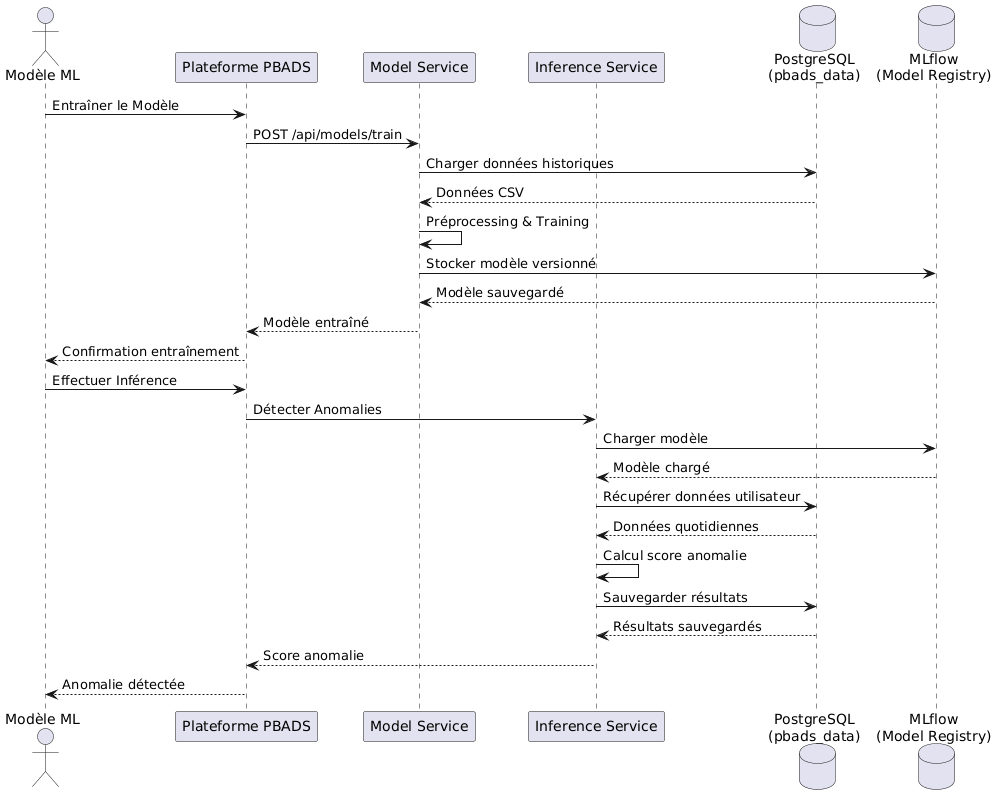
\includegraphics[width=\textwidth]{Figures/pbadsdiags/SequenceModelePlateformeDB.jpg}
    \caption{Diagramme de séquence - Modèle ML interagissant avec la base de données et la plateforme}
    \label{fig:seq_modele}
\end{figure}

\textbf{Scénario Modèle ML (Figure \ref{fig:seq_modele}) :} Ce diagramme détaille les interactions du modèle ML avec la plateforme et les bases de données. Le scénario commence par l'\textbf{entraînement du modèle} où le Model Service charge les données historiques depuis la base de données, effectue le preprocessing et l'entraînement, puis stocke le modèle versionné dans MLflow. Lors de l'\textbf{inférence}, le Inference Service charge le modèle depuis MLflow, récupère les données utilisateur depuis la base de données, calcule le score d'anomalie, et sauvegarde les résultats. Si une anomalie est détectée, une alerte est générée avec les détails de l'anomalie.

\section{Conclusion}

Ce chapitre a présenté la modélisation complète du système PBADS, couvrant l'analyse des besoins, la définition des objectifs, la méthodologie agile adoptée, et la modélisation conceptuelle détaillée avec les diagrammes UML. L'étude des lacunes des solutions existantes a permis d'identifier les besoins critiques en matière de détection automatique d'anomalies, de génération de recommandations personnalisées, et de visualisation interactive des données.

Les diagrammes UML (cas d'utilisation, classes et séquences) fournissent une vision claire de l'architecture et des interactions du système. Cette modélisation constitue la base solide pour l'implémentation technique qui sera détaillée dans le chapitre suivant.
